\chapter{Entwicklung der Schlüsselelemente}
\section{Übersicht des gesamten Modells}
Wie in Abbildung \ref{bild:tegglaoverview} zu erkennen, besteht das Fahrzeug aus vielen Einzelteilen. 
Auf die wichtigsten Komponenten, die in der Stückliste (Tabelle \ref{table:tegglaoverview}) genannt werden, wird in den folgenden Kapiteln genauer eingegangen.
\begin{figure}[!ht]
	\centering
	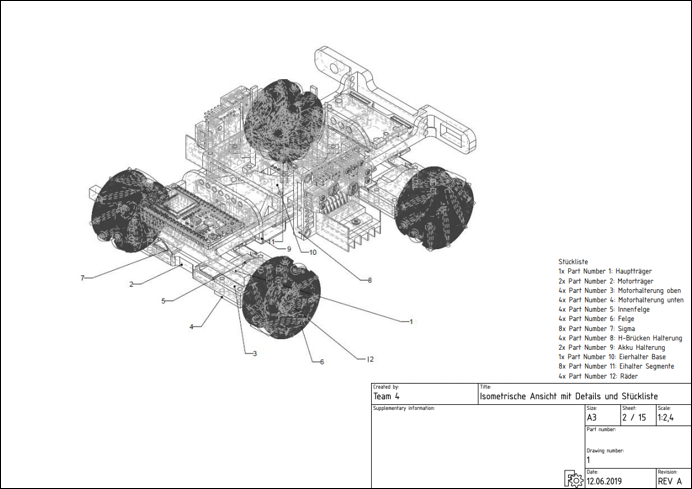
\includegraphics[width=\textwidth]{bilder/overview.png}
	\caption{Überischt der TEGGLA-Komponenten}
	\label{bild:tegglaoverview}
\end{figure}

\begin{table}[!ht]
\centering
\begin{tabular}{lr}
	Bezeichnung & Anzahl \\ 
	\midrule[3pt] 
	Hauptträger            & 1 \\ \midrule
	Motorträger            & 2 \\ \midrule
	Motorhalterung oben    & 4 \\ \midrule
	Motorhalterung unten   & 4 \\ \midrule
	Innenfelge und Felge   & 4 \\ \midrule
	Sigma                  & 8 \\ \midrule
	H-Brücken Halterung    & 4 \\ \midrule
	Akku Halterung         & 2 \\ \midrule
	Eihalterung Base       & 1 \\ \midrule
	Eihalter Segmente      & 8 \\ \midrule
	Mecanum-Räder          & 4
\end{tabular} 
\caption{Stückliste der TEGGLA-Komponenten} 
\label{table:tegglaoverview}
\end{table} 



\section{Schaltplan}
\begin{figure}[!ht]
	\centering
	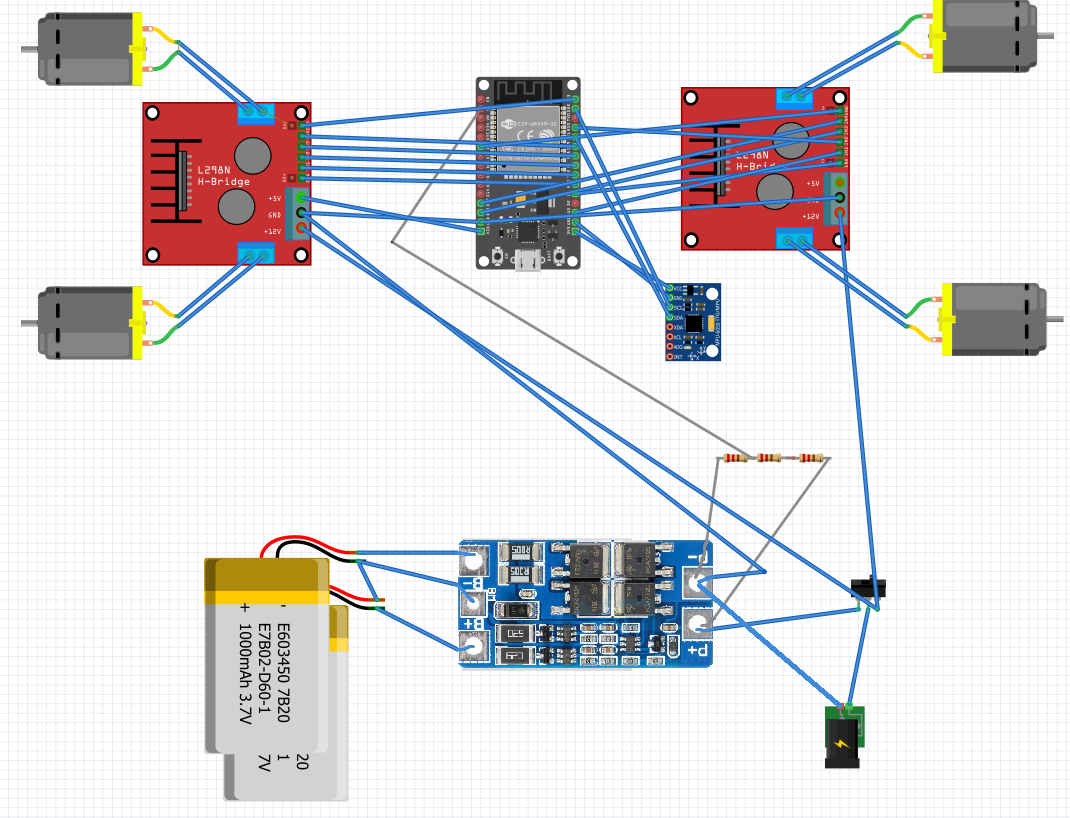
\includegraphics[width=\textwidth]{bilder/schaltplan.png}
	\caption{Schaltplan (gezeichnet mit Fritzing)}
	\label{bild:schaltpaln}
\end{figure}
Der Schaltplan (Abb~\ref{bild:schaltpaln}) zeigt eine grobe Skizze der Verkabelung des TEGGLA Fahrzeuges. Der 2S Lipo Akku wird hierbei durch die beiden Einzellenakkus dargestellt.
Der Hauptschalter, ein Dreipositionenschalter, dient zum Ein- und Ausschalten, sowie um das Fahrzeug in den Lademodus zu versetzen. 
Die linke der beiden H-Brücken dient neben der Motoransteuerung auch zur Spannungsregulierung für das ESP. 

Das ESP32 ist die zentrale Steuereinheit und steuert mit je sechs digitalen Pins die H-Brücken an und kann so die Motordrehrichtung sowie die Geschwindigkeit der Motoren steuern.
Das ESP32 kommuniziert auch via dem I2C Bus mit dem Gyroskop und versorgt dieses mit der 3.3V Spannungsversorgung.

Die Widerstände am Ausgang des BMS, auf welches im folgenden Abschnitt eingegangen wird, bilden einen 3:1 Spannungsteiler.
Dieser wird benötigt, da das ESP32 einen maximalen Spannungseingang von 3.3V verträgt, am BMS jedoch bis zu 9V anliegen können. Durch diesen Spannungsteiler ist es über den Analog-Digital-Wandler in dem ESP32 möglich, den Akkustand in 4095 Schritten auszulesen.
Hierduch wird dem User ein Feedback gegeben, wie lange die Akkuladung noch ausreicht.

\section{BMS und Laden}
Um einem Akkuschaden vorzubeugen, sollte ein User doch einmal übersehen, dass der Akku des Fahrzeugs leer ist, wurde ein BMS (Battery Management System) verbaut.
Dieses verhindert durch rechtzeitiges Abschalten ein Über- und Tiefenentladen des Akkus. 
Um das Fahrzeug wieder aufladen zu können, wurde ein externes Netzteil gekauft, welches über einen XT60 Stecker an das Fahrzeig angeschlossen werden kann.
Sobald der Hauptschalter in die Ladeposition gebracht wird, beginnt das Fahrzeug nun den internen Akku zu laden, bis das BMS bei geladenem Akku den Ladevorgang vollautomatisch beendet.

\section{Mecanum}
Als besonderes Merkmal des TEGGLA fallen sofort die besonderen Räder auf, die sogenannten Mecanum-Räder. 
Hierbei handelt es sich um von Bengt Ilon 1972 erfundene Räder, die es dem Fahrzeug erlauben sich in drei Freiheitsgraden zu bewegen.

Dies wird ermöglicht durch die um 45\degree{} gedrehten Rollen auf den Rädern, sodass diese wie ein X aussehen.
Durch unterschiedliche Drehrichtung und Drehgeschwindigkeit der Motoren kann das Fahrzeug in jegliche Richtungen innerhalb der Ebene bewegt werden. (vgl. Abb~\ref{bild:mecanum})

\begin{figure}[!ht]
	\centering
	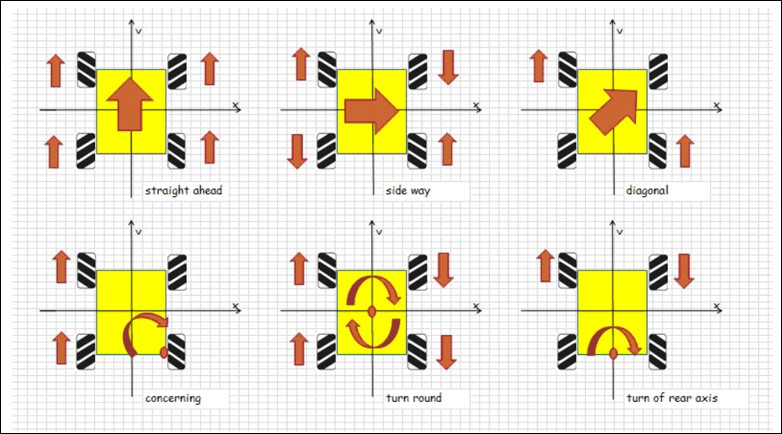
\includegraphics[width=\textwidth]{bilder/mecanum.jpg}
	\caption{Freiheitsgrade von Mecanum \cite{link:mecanum}}
	\label{bild:mecanum}
\end{figure}

Die jeweiligen Motorgeschwindigkeiten lassen sich hierbei durch Formeln~\ref{eq:mec1}--\ref{eq:mec2} berechnen.\\

$V_x =$ Motorgeschwindigkeit des x-ten Rads im Uhrzeigersinn (beginnend vorderes linkes Rad)\\
$V_d =$ gewünschte Roboter Geschwindigkeit $[-1, 1]$\\
$\theta_d =$ gewünschter Winkel $[0, 2\pi]$\\
$V_\theta =$ gewünschte Rotationsgeschwindigkeit $[-1, 1]$\\


\begin{align}
	V_1 = V_d\sin{(\theta_d+\frac{\pi}{4})} + V_\theta \label{eq:mec1}\\
	V_2 = V_d\cos{(\theta_d+\frac{\pi}{4})} - V_\theta\\
	V_3 = V_d\cos{(\theta_d+\frac{\pi}{4})} + V_\theta\\
	V_4 = V_d\sin{(\theta_d+\frac{\pi}{4})} - V_\theta \label{eq:mec2}
\end{align} 
\captionof{figure}{Formeln für die individuellen Motoren \cite{link:mecanum}}
\bigskip

Bei den in diesem Praktikum verwendeten Rädern handelt es sich um eine Modifizerung der STL Dateien von Jonah Innoart von dem Internetportal Thingiverse \cite{link:mecanum44}. 
In das Zentrum des Rades wurde mithilfe einer Boolean Operation von Blender3D eine Führung für die Getriebe geschnitten, sodass diese in das Rad eingeschoben werden können.

\section{Planetengetriebe}

Bereits in der 2. Woche des Projekts sind die ersten Entwürfe für die Planetengetriebe entstanden.
Dieser setzte sich aus zwei 3D-Modellen zusammen, dem Getriebe (Abb~\ref{bild:gearversion1-2}) und dem Rad, die beide von der Onlineplatform ``Thingiverse'' bezogen wurden.
Diese wurden in Blender zu einem Bauteil zusammenfügt (Abb~\ref{bild:gearversion1-1}). 

Nach einem erfolgreichen Testdruck stellte sich allerdings raus, dass das Getriebe zu viel Reibung hatte, sodass es nicht anlaufen konnte.

\begin{figure}[!ht]
	\centering
	\begin{subfigure}[b]{0.4\textwidth}
		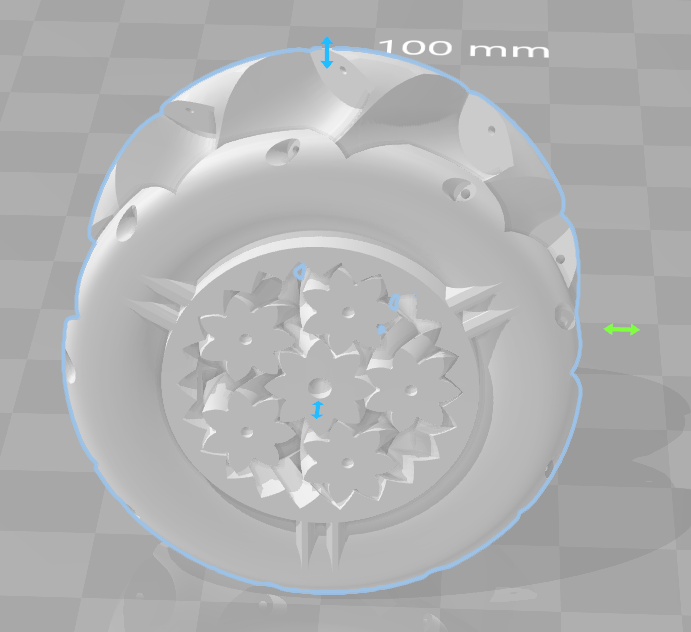
\includegraphics[width=\textwidth]{bilder/GetriebeVersion1-1.png}
		\caption{Version 1 des Planetengetriebes}
		\label{bild:gearversion1-1}
	\end{subfigure}
	\hspace{0.1\textwidth}%
	\begin{subfigure}[b]{0.4\textwidth}
		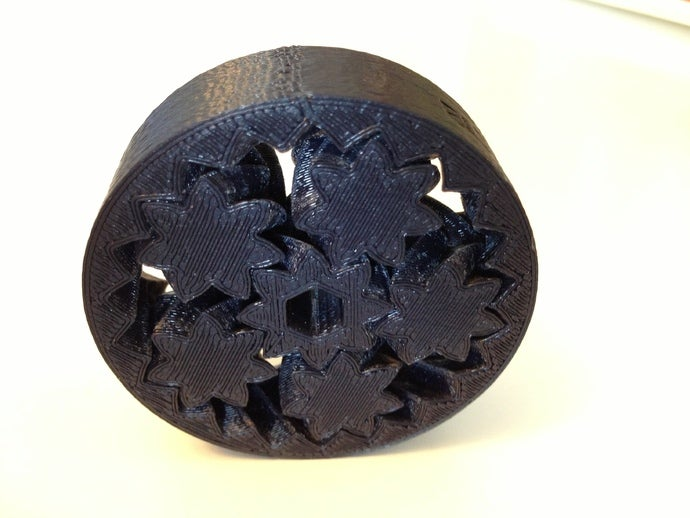
\includegraphics[width=\textwidth]{bilder/GetriebeVersion1-2.jpg}
		\caption{Orginal des verwendeten Planetengetriebes \cite{link:planetgear1}}
		\label{bild:gearversion1-2}
	\end{subfigure}
\end{figure}

Um der Reibung entgegen wirken zu können, wurden im nächsten Schritt mit dem CAD Programm ``OpenSCAD'' (Abb~\ref{bild:gearversion2}) eigene Planetengetriebe erstellt.
Hierbei lassen sich vielerlei Parameter einstellen, beispielsweise Größe, Toleranzen, Zahnzahl, Planetenzahl, etc.
Dies ermöglicht frei mit der Übersetzung sowie den druckbaren Toleranzen zu testen um das bestmögliche Getriebe zu bekommen.
\begin{figure}[!ht]
	\centering
	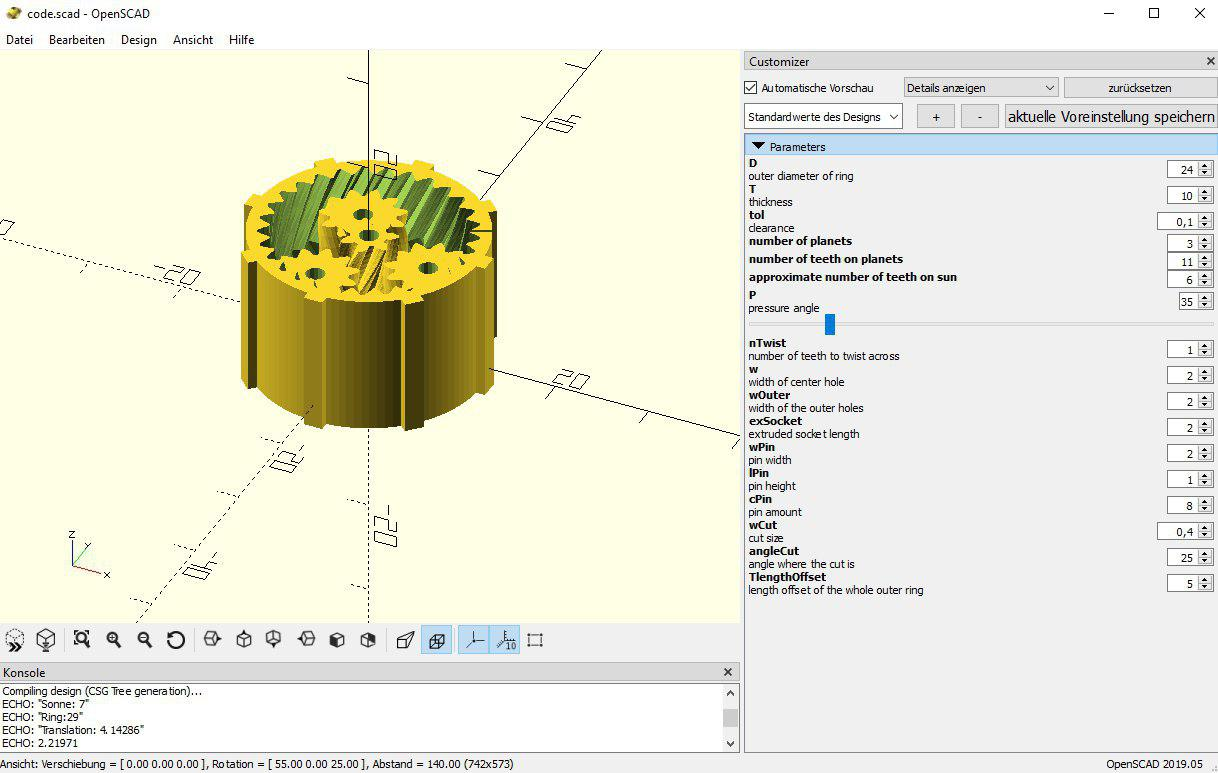
\includegraphics[width=0.7\textwidth]{bilder/GetriebeVersion2.jpg}
	\caption{OpenSCAN zum Erstellen von Planetengetrieben}
	\label{bild:gearversion2}
\end{figure}

Durch die Funktionsweise von Additiver Fertigung lassen sich V-förmig verzahnte Getriebe als eine Einheit drucken.
Dies wäre mit konventionellen Fertigungsprozessen nicht möglich.
Da jedoch aufgrund von mangelnder Genauigkeit des 3D Druckers die Toleranzen so hoch gewählt werden müssen, 
sodass sich die Zahne nicht verschmelzen, führt dies zu viel Spiel in dem Getriebe.

Um jedoch das Getriebe weiterhin platzsparend in das Rad zu senken, wurde hier ebenfalls mit geradverzahnten Getrieben (Abb.~\ref{bild:getrgerade}) getestet.
Hierbei entsteht jedoch das Problem der Fixierung der Planeten. Es entstand somit der Plan eine Gegenfelge zu Benutzten um alle Teile zu halten.

\begin{figure}[!ht]
	\centering
	\begin{subfigure}[b]{0.4\textwidth}
		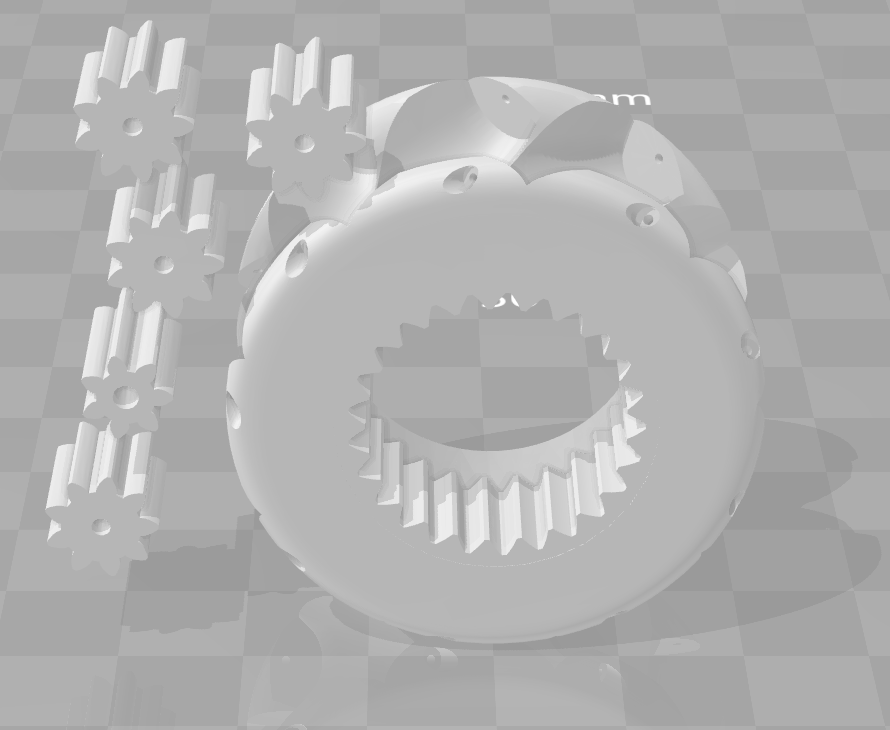
\includegraphics[width=\textwidth]{bilder/GetriebeVersion3-1.png}
		\caption{Version 2 des Planetengetriebes}
		\label{bild:gearversion3-1}
	\end{subfigure}
	\hspace{0.1\textwidth}%
	\begin{subfigure}[b]{0.4\textwidth}
		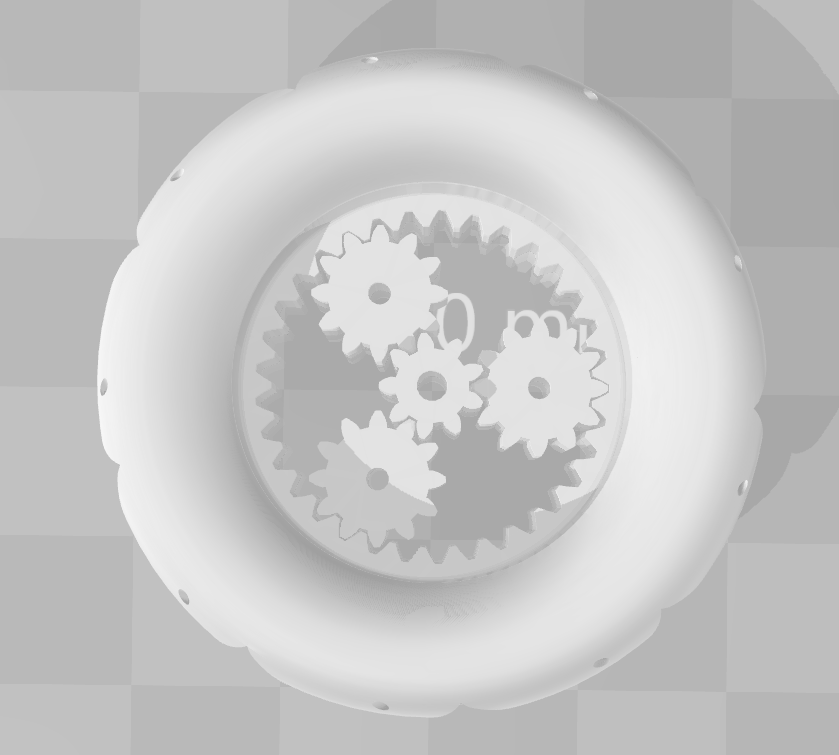
\includegraphics[width=\textwidth]{bilder/GetriebeVersion3-2.png}
		\caption{Version 3 des Planetengetriebes}
		\label{bild:gearversion3-2}
	\end{subfigure}
	\caption{Im Rad integrierte Getriebe}
	\label{bild:getrgerade}
\end{figure}

Weiterhin gab es noch das Problematik der zu niedrigen Übersetzungen. 
Hier hat es einige Iterationen gedauert bis eine Übersetzung von über 1:4 erreicht werden konnte.

Probleme die hier aufgetreten sind, sind beispielsweise zu kleine Zähne (Abb.~\ref{bild:gearversion4-1}), sodass diese nicht mehr ineinander greifen konnten.

Desweiteren hängt die mögliche Übersetzung auch von der Anzahl der Planeten ab. 
Sind zu viele Planeten im Ring (Abb.~\ref{bild:gearversion4-3}) überschneiden sie sich, und man muss somit auf weniger Planeten (Abb.~\ref{bild:gearversion4-2}) zurückgreifen, was die Stabilität beeinträchtigt.
Hierbei lässt sich auch der Kraftwinkel der Zähne einstellen. 
Ist der Winkel zu niedrig (Abb.~\ref{bild:gearversion4-4}) rutschen die Zähne einfacher durch, verhaken sich jedoch nicht so stark.

\begin{figure}[!ht]
	\centering
	\begin{subfigure}[b]{0.4\textwidth}
		
\includegraphics[width=\textwidth]{bilder/GetriebeVersion4-1.png}
		\caption{Version 4 des Planetengetriebes}
		\label{bild:gearversion4-1}
	\end{subfigure}
	\hspace{0.1\textwidth}%
	\begin{subfigure}[b]{0.4\textwidth}
		
\includegraphics[width=\textwidth]{bilder/GetriebeVersion4-2.png}
		\caption{Version 5 des Planetengetriebes}
		\label{bild:gearversion4-2}
	\end{subfigure}


	\begin{subfigure}[b]{0.4\textwidth}
		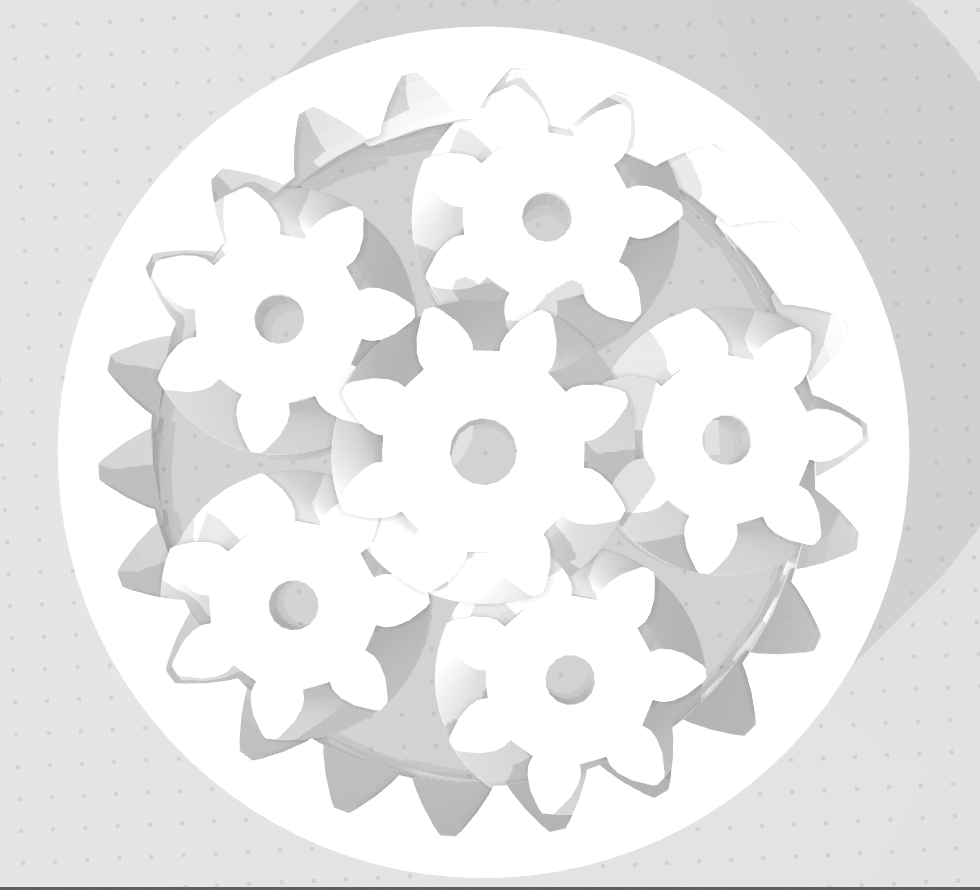
\includegraphics[width=\textwidth]{bilder/GetriebeVersion4-3.png}
		\caption{Version 6 des Planetengetriebes}
		\label{bild:gearversion4-3}
	\end{subfigure}
	\hspace{0.1\textwidth}%
	\begin{subfigure}[b]{0.4\textwidth}
		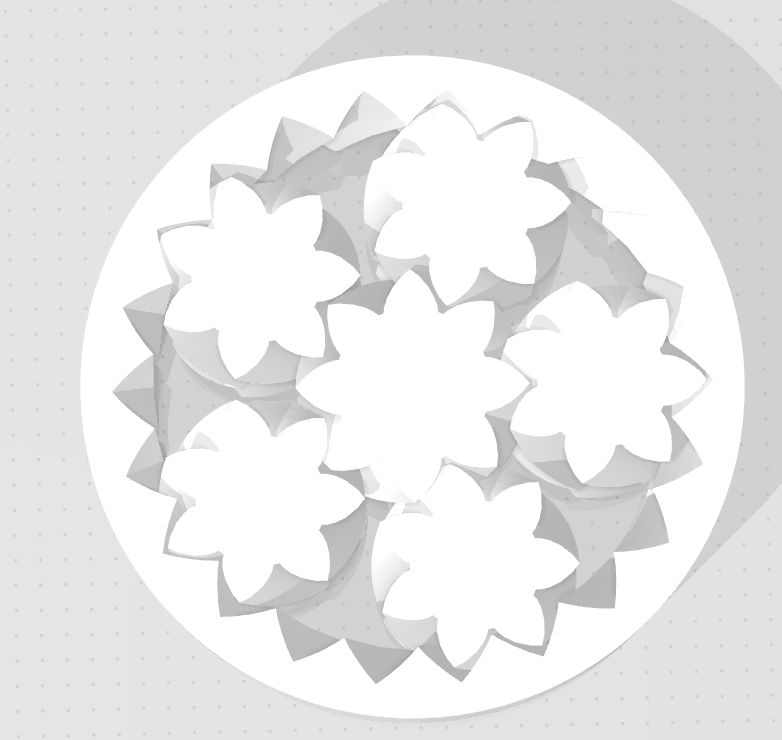
\includegraphics[width=\textwidth]{bilder/GetriebeVersion4-4.png}
		\caption{Version 7 des Planetengetriebes}
		\label{bild:gearversion4-4}
	\end{subfigure}

	\caption{Iterationen der Getriebe}
\end{figure}

Da Versuche mit höheren Übersetzungen als 1:4 nie Erfolg hatten, wurden ebenfalls mehrstufige Getriebe (Abb.~\label{bild:compgetr}) getestet, sogenannten ``Composite Gear Sets''.
Hierbei sind Übersetzungen von über 1:66 möglich, was für diese Anwendung perfekt wäre. 
Selbst bei mehrfachen Testdrucken der Zweistufigen Getriebe gelang es nicht, ein lauffähiges Getriebe mit ausreichendem Wirkungsgrad zu erreichen.
Es gelang bei einigen Getrieben sie per Hand mit einiger Gewalt zu drehen, jedoch hatten die Motoren nicht genung Moment um überhaupt aus dem Stillstand loszudrehen.

\begin{figure}[!ht]
	\centering
	\begin{subfigure}[b]{0.4\textwidth}
		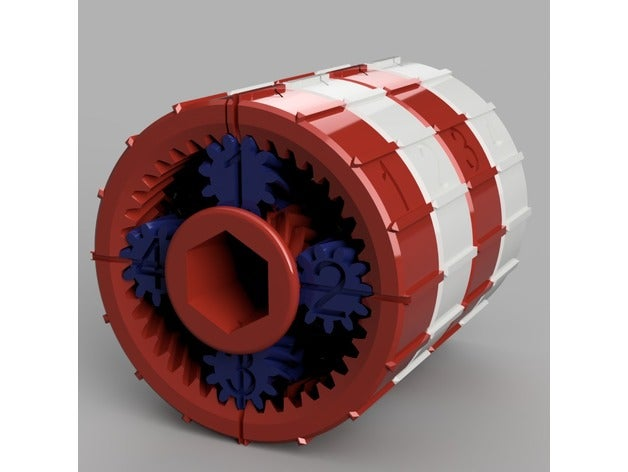
\includegraphics[width=\textwidth]{bilder/GetriebeVersion5-1.jpg}
		\caption{Version 8 des Planetengetriebes \cite{link:planetgear5-1}}
		\label{bild:gearversion5-1}
	\end{subfigure}
	\hspace{0.1\textwidth}%
	\begin{subfigure}[b]{0.4\textwidth}
		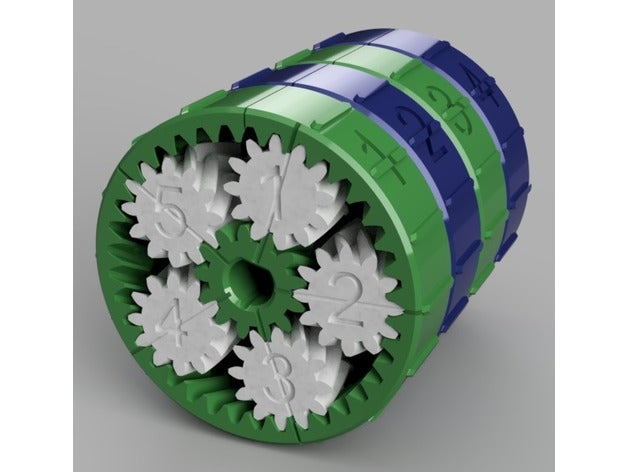
\includegraphics[width=\textwidth]{bilder/GetriebeVersion5-2.jpg}
		\caption{Version 9 des Planetengetriebes \cite{link:planetgear5-2}}
		\label{bild:gearversion5-2}
	\end{subfigure}
	\caption{Mehrstufige Getriebe}
	\label{bild:compgetr}
\end{figure}

Aus diesen Gründen wurde sich letztendlich auf einstufige Getriebe mit einer Übersetzung von $1:4.14$ geeinigt.
Obwohl dies zwar nicht ausreichend ist, um die Motoren von einer Lastdrehzahl von bis zu 6000 rpm auf eine lenkbare Geschwindigkeit zu übersetzen,
wurde hier ebenfalls mit bedacht, dass weitere Steurung durch Software mithilfe der H-Brücken möglich ist.

Dies führt zu dem finalen Design (Abb.~\ref{bild:currGetr}). 
Aufgrund der geringeren Reibung wurde sich hierbei für eine Geradverzahnung entschieden.
Der 14mm lange Ring ist an einer Seite offen, sodass er aufgebogen werden kann um ihn um den Käfig (Abb.~\ref{bild:currKaefig}) zu schließen.
Bei dem Käfig handelt es sich um eine Verbindung der Innenfelge, die auf den Motor aufgesteckt wird mit der Außenfelge.
Der Käfig erfüllt ebenfalls den Zweck die Planeten an ihrem Platz zu halten, sowie zusätzliche Stabilität der Achsen zu gewährleisten.
Für die Achsen der Planeten dienen hier 1.5mm, die auf der Innenseite eingeklebt sind.

\begin{figure}[!ht]
	\centering
	\begin{subfigure}[b]{0.4\textwidth}
		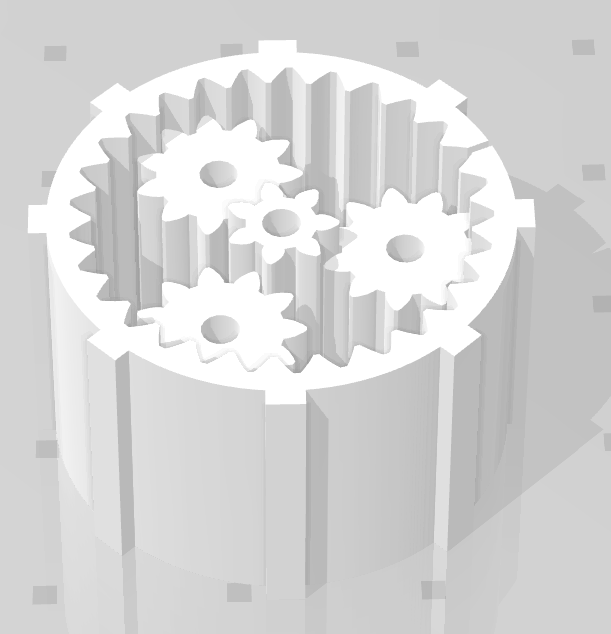
\includegraphics[width=\textwidth]{bilder/currGetr.png}
		\caption{Finale Version des Planetengetriebes}
		\label{bild:currGetr}
	\end{subfigure}
	\hspace{0.1\textwidth}%
	\begin{subfigure}[b]{0.4\textwidth}
		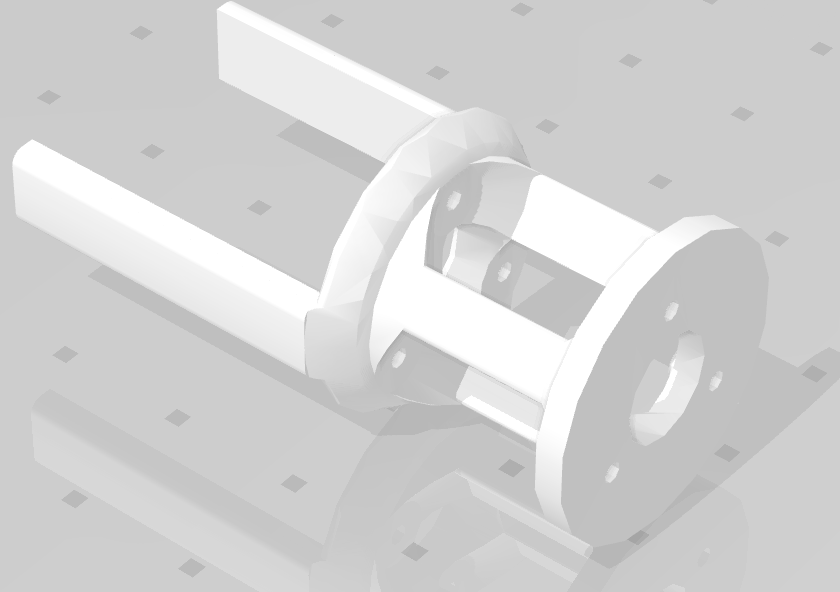
\includegraphics[width=\textwidth]{bilder/currKaefig.png}
		\caption{Finale Version des Käfigs}
		\label{bild:currKaefig}
	\end{subfigure}
	\caption{Finale Getriebebaugruppe}
\end{figure}


\section{ESP-32 vs. ESP-8266}
Bei dem vom Lehrstuhl gestellten ESP-8266 handelt es sich um einen WiFi-fähigen Microcontroller der chinesischen Firma ``espressif''.
Dieser besitzt 17 GPIO Pins, wovon jedoch lediglich 11 Pins nutzbar sind, da 6 an den externen SPI Flash angeschlossen sind.
Da dies wie in Tabelle~\ref{table:pins} aufgezeigt nicht für unsere Zwecke reicht, musste auf den leistungsstärkeren ESP-32 ausgewichen werden.

\begin{table}[!ht]
\centering
\begin{tabular}{lr}
	\multicolumn{2}{c}{Benötigte Pins} \\ 
	\midrule[3pt] 
	4x PWM & Motor Enable \\ 
	\midrule 
	8x Output & Motor Richtung \\ 
	\midrule 
	2x I$^2$C & Gyroskop \\ 
	\midrule 
	1x ADC & Batteriespannung \\ 
	\midrule
	\midrule 
	\multicolumn{2}{c}{15 Pins} \\ 
	 
\end{tabular} 
\caption{Aufzählung benötigter Pins} 
\label{table:pins}
\end{table} 

Obwohl die Anzahl der Pins das ausschlaggebende Argument für einen Austausch des MicroControllers war, bringt dieser natürlich weitere Vorteile mit sich.

Beispielsweise profitiert die später genauer erklärte Website stark davon, auf einen zweiten Core ausgelagert werden zu können.

Siehe Tabelle~\ref{table:esp32} für einen Vergleich der beiden MicroController anhand der für dieses Projekt relevanten Faktoren.


\begin{table}[!ht]
\centering	
\begin{tabular}{lcc}
	& ESP-8266 & ESP-32 \\ 
	\midrule[3pt]
	Cores & single core & dual core \\ 
	\midrule
	Max Frequenz & 160 MHz & 240 MHz \\ 
	\midrule 
	\textbf{GPI} & \textbf{17 (11 nutzbar)} & \textbf{36 (30 nutzbar)} \\ 
	\midrule
	SRAM & 160 KB & 520 KB \\ 
	\midrule
	ADC Auflösung & 10 bit & 12 bit \\ 
	\midrule
	Stromverbrauch & 80 mA & 260 mA \\ 
	\midrule
	Preis (aus China) & \EUR{2} & \EUR{4} \\ 
\end{tabular} 
\caption{Vorteile des ESP-32} 
\label{table:esp32}
\end{table} 


\section{User-Interface}
Eine passende, nutzerfreundliche und optisch ansprechende UI hatte für das Projekt TEGGLA von Anfang an eine hohe Priorität. Es wurden zwei verschiedene UIs für das Projekt entwickelt, welche nachfolgend detailliert beschrieben werden. 

\subsection{Java (obsolet)}
Das erste Konzept für eine passende UI wurde mit Java entwickelt. 
Java (und das Framework Java Swing) bieten grundsätzlich einige Möglichkeiten Benutzeroberflächen zu bauen und da Java eine der meistgenutzten Programmiersprachen ist, haben wir uns vorerst dafür entschieden.

Die Java UI besteht aus zwei Fenstern, welche vorerst die Verbindung zum TEGGLA sicherstellen und anschließend die Steuerung und Kommunikation ermöglichten.

\begin{figure}[!ht]
	\centering
	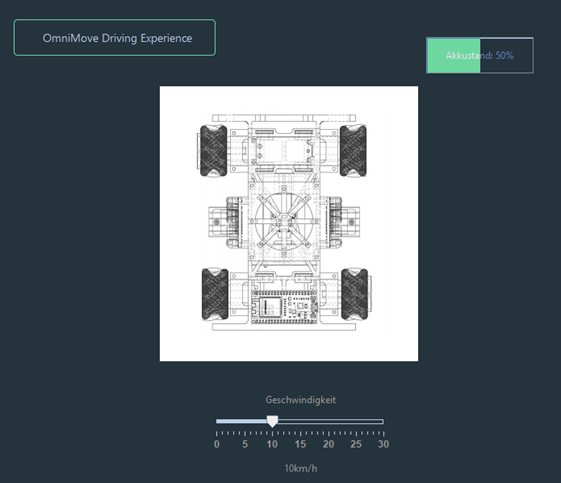
\includegraphics[width=\textwidth]{bilder/java1.png}
	\caption{Java Fenster 1: Verbindungsaufbau}
	\label{bild:java1}
\end{figure}


Im ersten Fenster (Abb.~\ref{bild:java1}) müssen in die Textfelder „IP Adresse“ und „PORT“ die passenden Daten eingegeben werden, um anschließend mit dem „Connect“ Button eine Verbindung zum TEGGLA aufzubauen. 
Falls das nicht gelungen ist, bekommt der Nutzer eine Fehlermeldung als Pop-Up und muss die Daten erneut eingeben. 
Im Erfolgsfall erscheint eine kurze Erfolgsmeldung und es öffnet sich das zweite Fenster.

\begin{figure}[!ht]
	\centering
	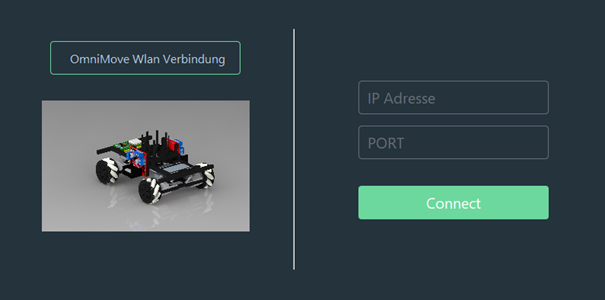
\includegraphics[width=\textwidth]{bilder/java2.png}
	\caption{Java Fenster 2: Steuerung}
	\label{bild:java2}
\end{figure}

Im zweiten Fenster (Abb.~\ref{bild:java2}) werden alle wichtigen Daten für die Steuerung
und Kommunikation des TEGGLA angezeigt, nämlich Geschwindigkeit und Akkustand.

Die Entwicklung des zweiten Fensters war noch nicht ganz abgeschlossen, als Java
durch die Verwendung der neuen UI mit JavaScript / HTML5 abgelöst wurde. Daher
wäre dieses Fenster noch durch die Visualisierung der Motoransteuerung und –
auslastung ergänzt worden.\\

Abschließend lässt sich festhalten, dass die Entwicklung einer UI mit Java (und Java Swing) durchaus Vorteile hat, aber das Erstellen einer optisch ansprechenden Benutzeroberfläche sehr zeitaufwändig ist. 
Für diese zwei Fenster (mit Logikschicht) wurden in etwa 1000 Zeilen Quellcode benötigt, was für größere Projekte mit mehr Komponenten nicht empfehlenswert ist. 
Der zugehörige Quellcode ist im Anhang des Berichts und kann bei Interesse daher noch genauer betrachtet werden.



\subsection{HTML5 und Controller-Anbindung}

Das Java Programm wurde aus mehreren Gründen zugunsten einer auf HTML5 sowie JavaScript basierten Weboberfläche ersetzt:\par

\begin{itemize}
	\item Native und einheitliche Unterstützung für Controller unterschiedlichster Marken in HTML5\par
	
	\item Unabhängig von Java Laufzeitumgebung, sowie Verfügbarkeit des Programms.\\
	(Hierbei muss nur ein Browser auf dem PC installiert sein.)\par
	
	\item Einfache Übertragung der Daten per WebSockets anstatt von ``raw''  Sockets, ohne ein eigenes ``Frame'' um die Daten bauen zu müssen
\end{itemize}\par


\vspace{\baselineskip}
Die Erstellung der Website lässt sich sehr leicht durch die ESPAsyncWebServer Library für den ESP32 lösen. \par

Diese hostet direkt auf dem ESP32 einen WebServer der sowohl HTML5, JS, als auch CSS bereitstellen kann. Als Speicherort für diese Dateien wird das sogenannte Dateisystem SPIFFS verwendet, welches den Flashspeicher des ESP32 als Dateisystem benutzt, wie es beispielsweise aus Windows bekannt ist.\par

Eine Einschränkung ist die Limitierung auf eine gleichzeitige Verbindung zu dem Server. 
Dies wurde empirisch herausgefunden und somit konnte nicht sicher gesagt werden, ob es sich hier um eine Einschränkung aufgrund mangelnder Rechenleistung handelt oder ob die Library nicht mehr gleichzeitige Verbindungen unterstützt. Als Lösung dieses Problems, wurde nun die Anzahl der Verbindungen, die der WiFi Accesspoint akzeptiert, auf eins gesetzt.\par


\vspace{\baselineskip}

\begin{figure}[!ht]
	\centering
	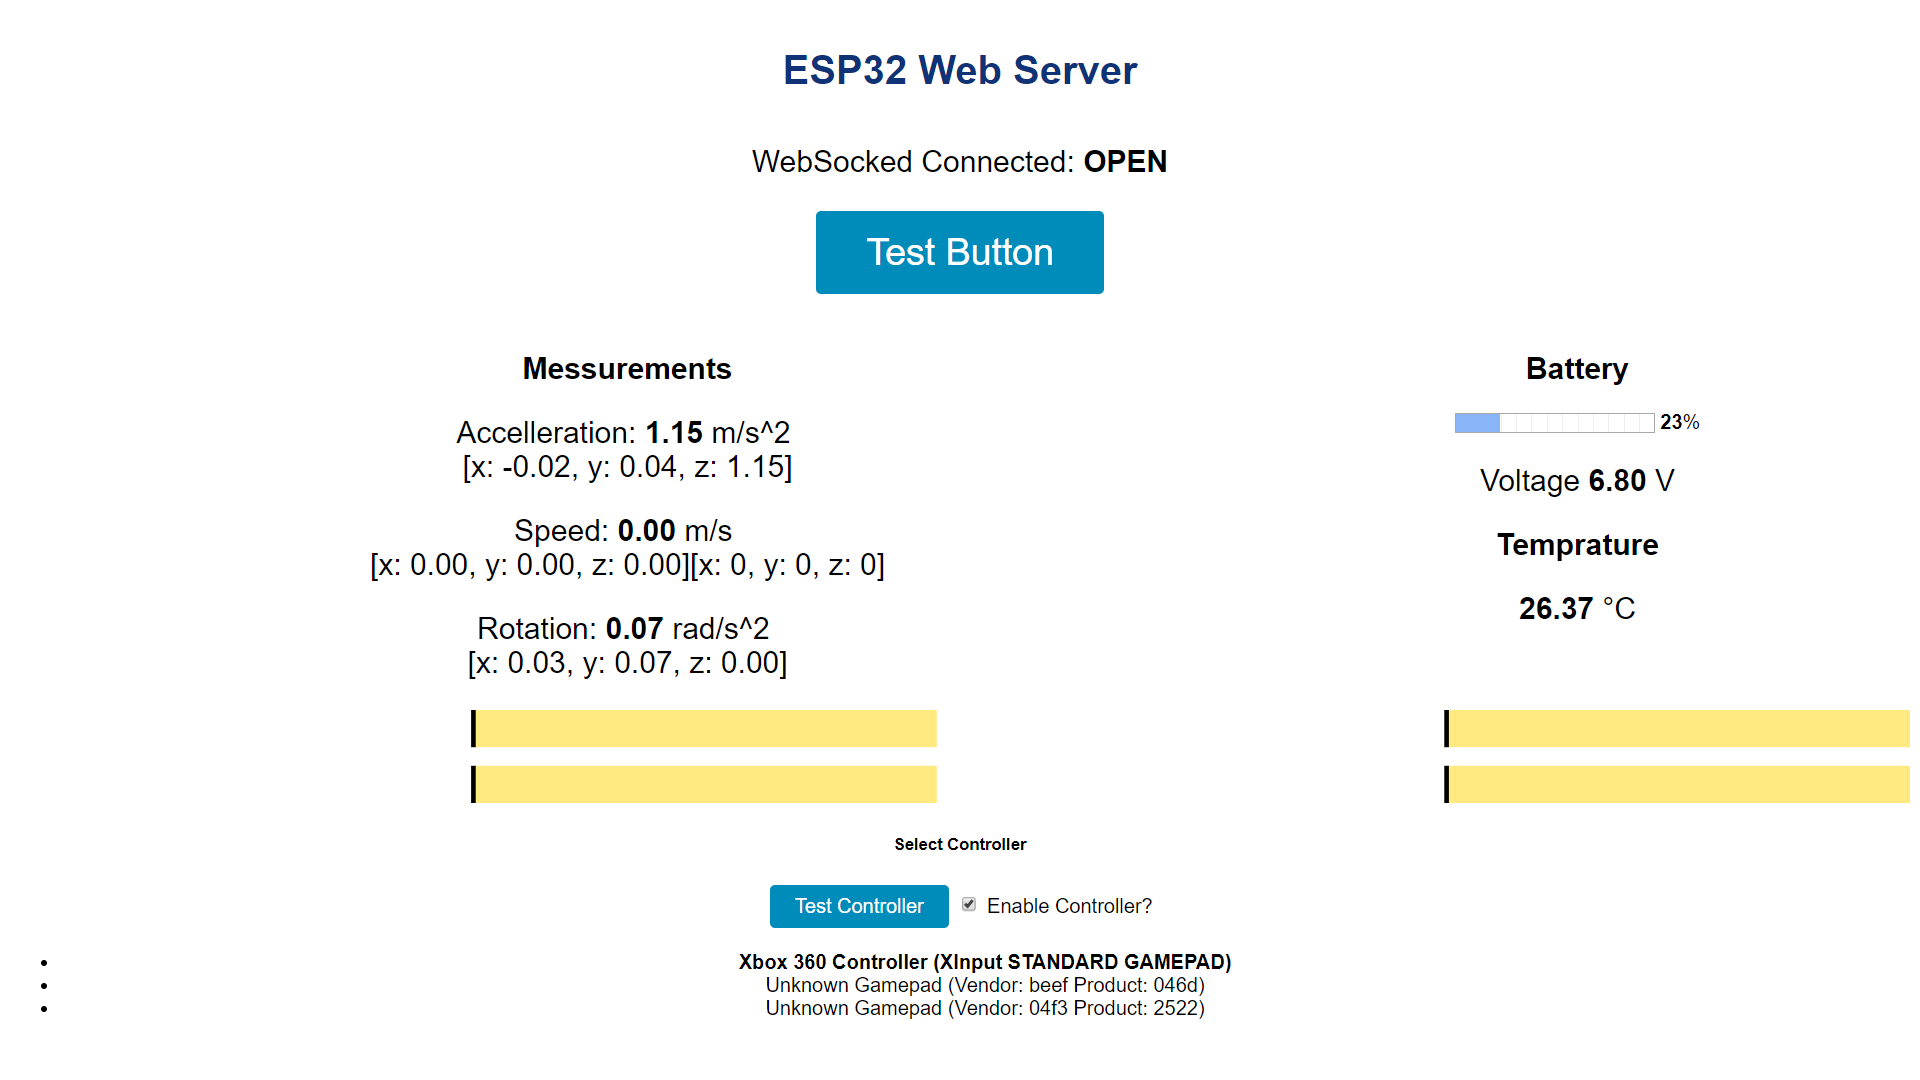
\includegraphics[width=\textwidth]{bilder/WebValues.png}
	\caption{Bildschirmfoto Weboberfläche}
	\label{bild:webvalues}
\end{figure}

In der Weboberfläche (Abb.~\ref{bild:webvalues}) sind ebenfalls noch jegliche Messwerte hinterlegt, die das Fahrzeug sammelt.\par

Diese sind:\par

\begin{itemize}
	\item Beschleunigung 
	\item Geschwindigkeit
	\item Rotationsgeschwindigkeit
	\item Batteriespannung
	\item Temperatur
	\item Drehgeschwindigkeit der jeweiligen Motoren
\end{itemize}\par


\vspace{\baselineskip}
Für die Wahl des Controllers ist eine auswählbare Liste aller angeschlossenen Controller am Ende der Seite vorhanden. Falls der Nutzer keinen Controller besitzt oder angeschlossen hat, kann durch das Abwählen der Checkbox auf die Steuerung per WASD, sowie die Pfeiltasten gewechselt werden.\par

\subsection{Protokoll}
Zum Übertragen wurde ein binäres Protokoll (Tabelle~\ref{table:protokoll}) entwickelt, um die Datenrate gering zu halten, sowie die Verarbeitung auf dem Microcontroller zu vereinfachen.\par

Da durch Websockets bereits ein Integrierter Frame geschickt wird, muss nicht bei jeder Nachricht die Länge sowie Anfangs- und Endbyte mitgeschickt werden, wie es sonst bei raw Sockets nötig gewesen wäre.\par

Hierbei wird jeder Wert als Int16 geschickt, um ein ausreichend großes Spektrum bei geringer Datenrate zu gewährleisten. \par

Am Anfang jeder Nachricht wird die ID ebenfalls als int16 geschickt, somit wären 65536 unterschiedliche Nachrichten erlaubt.\par

Um die Anzahl an Nachrichten zu verringern, wurden die Batteriespannung und Werte des Gyroskop zu einer kombinierte Nachricht zusammengefasst, um den Overhead gering zu halten.\par

\begin{table}[ht]
	\centering
	\resizebox{\textwidth}{!}{
\begin{tabular}{|c|c|c|c|c|c|c|c|c|c|c|c|c|}
	\hline 
	\textbf{Name} & \textbf{ID} & \multicolumn{11}{c|}{\textbf{Werte}} \\ 
	\hline 
	\hline 
	DRIVE & 0 & X-Achse L & Y-Achse L & X-Achse R & Y-Achse R &  &  &  &  &  &  &  \\ 
	\hline 
	GYRO & 1 & Speed-X & Speed-Y & Speed-Z & Accel-X & Accel-Y & Accel-Z & Rot-X & Rot-Y & Rot-Z  &  & \\ 
	\hline 
	BATTERY & 2 & Voltage &  &  &  &  &  &  &  &  &  &  \\ 
	\hline 
	MOTOR & 3 & Speed-M1 & Speed-M2 & Speed-M3 & Speed-M4 &  &  &  &  &  &  &  \\ 
	\hline 
	COMB & 4 & Speed-X & Speed-Y & Speed-Z & Accel-X & Accel-Y & Accel-Z & Rot-X & Rot-Y & Rot-Z  & Battery & Temp \\ 
	\hline 
\end{tabular}} 
\caption{Binäres Protokoll} 
\label{table:protokoll}
\end{table} 



\section{Steuerung per (XBox) Controller}
Wie bereits in der Dokumentation der Weboberfläche erwähnt, wird die Steuerung primär per Spiele Controller gelöst, beispielsweise einem XBox-Controller von Microsoft.
Diese Entscheidung ist durch die erhöhte Mobilität motiviert. 

Mit einer Steurung per WASD bzw. per Pfeiltasten sind nur binäre Zustände messbar, gedrückt oder nicht gedrückt, volle Geschwindigkeit oder Stillstand.
Im Vergleich dazu erlauben uns die JoySticks des Controllers durch unterschiedlich starke Auslenkung die Geschwindigkeit sehr variabel zu bestimmen.

Da hierbei ebenfalls der JoyStick in jegliche Richtungen bewegt werden kann, können ebenfalls die Mecanum-Räder so angesteuert werden, dass sie in genau diese Richtung fahren.

Jedoch sind hiermit nur zwei der drei Freiheitsgrade unseres Fahrzeugs abgedeckt. Um Rotationen um die eigene Achse mit variabler Geschwindigkeit zu steuern, wird die Eingabe des linken und des rechten JoySticks mit folgenden Formeln überlagert.

\bigskip
Sei hier $controlSide$ Auslenkung des linken Sticks in X Richtung (nach rechts), 
$controlFront$ Auslenkung des linken Sticks in Y Richtung (nach vorne) und 
$controlTurn$ Auslenkung des rechten Sticks in X Richtung (nach rechts), 

\begin{align}
	\theta &= atan2(controlSide, controlFront)\\
	V_d &= min(\sqrt{controlFront^2 + controlSide^2}, 1023) - \frac{controlTurn}{2}\\
	V_\theta &= \frac{controlTurn}{2}
\end{align}


\section{PLA vs. TPU}
Der Großteil der Teile für den TEGGLA wurde mit PLA Filament gedruckt. 
PLA steht für Polyactide, TPU steht für thermoplastisches Polyurethan. 
In diesem Kapitel wird auf die Unterschiede zwischen TPU und PLA eingegangen. 

PLA hat im Vergleich ein höheres E-Modul, was zu einer höheren Zugfestigkeit und Steifigkeit führt. 
Auch in Sachen Verarbeitung ist PLA deutlich einfacher als TPU. 
Im Gegensatz zu TPU ist der Druckprozess mit PLA problemlos. 
Darüber hinaus ist TPU ein bisschen teurer als PLA. 

Warum also TPU? TPU ist im Vergleich zu PLA viel flexibler und elastischer. 
Deswegen fiel die Wahl beim Rohstoff für die Sigmas und die Motorhalterungen auf TPU. 
Acht Sigmas verbinden die zwei Motorträger mit dem Hauptträger. 
Sie dienen hier quasi als Federung für die beiden ``Achsen''. 
Die Motorhalterungen sind das Bindeglied zwischen Motor und Motorträger. 
Es ist naheliegend, eine Federung und eine Befestigung für die Motoren aus einem elastischen Material zu drucken, auch wenn man mit einigen Nachteilen leben muss.

Um ein ansprechendes Design zu erhalten und um die Unterscheidung der Materialien zu erleichtern, wurde für den Robter, sowie in den Skizzen, für PLA die Farbe schwarz verwendet, für TPU die Farbe weiß.


\section{Eierhalter}					
Der Leichtbau-Anspruch lässt sich bei allen Komponenten des TEGGLA wiederfinden, sogar beim Eierhalter. 
Dieser wurde aus mehreren einzelnen Bauteilen erstellt, um mit möglichst wenig Gewicht die größte Stabilität für das Ei zu erreichen. 
Es wurde vorerst das Fundament des Eihalters gedruckt und anschließend mit 8 Eihalter-Segmenten verbunden. 
Somit kann das zu transportierende Ei schnell und sicher auf dem TEGGLA verwahrt werden. 

Zusätzlich befindet sich der Eierhalter genau im Schwerpunkt des Fahrzeugs, um sicherzustellen, dass die aufgenommene Last gleichmäßig verteilt werden kann und die omnidirektionale Fahrweise des TEGGLA nicht beeinträchtigt werden kann.



\section{Leichtbau}	

Bei der Konstruktion des TEGGLA wurde auf die Verwendung von massiven und schweren Bauteilen komplett verzichtet, wodurch das geringe Gesamtgewicht des Fahrzeugs (ca. 500 Gramm) erreicht worden ist. 
Dabei sind die schwersten Bauteile die Elektronikbauteile, auf die kein Einfluss genommen werden kann, wie die Motoren (je 36g), die H-Brücken (je 25g) sowie der Akku (62g). 

Um ein omnidirektionales Fahren zu ermöglichen, benötigt der TEGGLA vier Motoren und zwei H-Brücken, welches das Gewicht des Fahrzeugs im Vergleich zu konventionellen Fahrzeugen erhöht. 
Die Leichtbau Anforderung ist daher in gewisser Weise in Konflikt mit einer innovativen Idee, schnellem Fahren und vor allem dem omnidirektionalen Fahren. 

Durch die Verwendung einer elastischen Federung konnte auf ein Gehäuse für den Schutz der Elektronik verzichtet werden und zusätzlich konnten die dadurch entstandenen Hohlräume für technische Bauteile und Verbindungskabel genutzt werden.    
